\documentclass[a4paper]{article}

\usepackage{INTERSPEECH2016}
\usepackage{graphicx}
\usepackage{amssymb,amsmath,bm}
\usepackage{textcomp}
\usepackage{epsfig,amsmath,rotating,latexsym,comment}
\usepackage{subfigure,tabularx,tabulary,caption,float}
\usepackage{enumitem} % remove tab for bullet points during itemize
\usepackage[noadjust]{cite} % to produce ranges [1]-[3] instead of [1],[2],[3] and to sort the order
\usepackage{color}
\usepackage{tikz}
\usepackage{tipa}\newcommand{\ipa}[1]{\textipa{#1}}
\usepackage{stackrel}
\usepackage{fnpct} % use footnote in Tab or Fig caption
\usepackage{url}
\usetikzlibrary{positioning,shadows,arrows,shapes,calc}
%\usepackage{graphicx,pstricks}
%\usepackage{cases}
\def\vec#1{\ensuremath{\bm{{#1}}}}
\def\mat#1{\vec{#1}}
\DeclareMathOperator*{\argmax}{arg\,max}
\DeclareMathOperator*{\argmin}{arg\,min}
\newcommand{\mytikzscale}{0.9}
\newcommand{\myvspacefig}{\vspace{-4mm}}

\sloppy % better line breaks
\ninept

\title{Automatic speech recognition using probabilistic transcriptions in Swahili, Amharic, and Dinka}

\makeatletter
\def\name#1{\gdef\@name{#1\\}}
\makeatother \name{{\em Amit Das$^\star$\thanks{$^\star$first authors}, Preethi Jyothi$^\star$, Mark Hasegawa-Johnson\footnotemark[1]}}

\address{Department of Electrical and Computer Engineering \\
University of Illinois at Urbana-Champaign \\
Illinois, IL 61801, USA \\
{\small \tt \{amitdas, pjyothi, jhasegaw\}@illinois.edu}}

\begin{document}
\maketitle

\begin{abstract}
In this study, we develop automatic speech recognition systems for three sub-Saharan African languages
using probabilistic transcriptions collected from crowd workers who neither speak nor have any familiarity 
with the African languages. There is a language mismatch in this scenario. More specifically, utterances spoken in African languages were transcribed by crowd workers who were mostly native speakers of English. Due to this, such transcriptions are highly prone to inaccuracies in labels. The three African languages in consideration are Swahili, Amharic, and Dinka. First, we use a recently introduced technique called mismatched crowdsourcing which processes the raw crowd transcriptions through merging, contextual weighting, and ranking. Next, we  adapt multilingual HMM and DNN systems using the probabilistic transcriptions of the African languages.  Finally, we report the results using both deterministic and probabilistic phone error rates. Automatic speech recognition systems developed using this recipe are particularly useful for low resource languages where there is limited access to linguisitc resources and/or transcribers in the native language.
\end{abstract}
%
\noindent{\bf Index Terms}: mismatched crowdsourcing, cross-lingual speech recognition, deep neural networks,
African languages
\vspace{-3mm}
%
\section{Introduction}  \vspace{-2mm}
\label{sec:Introduction}
This work is focussed on knowledge transfer from multilingual data collected from a set of source (train) languages to a target (test) language that is mutually exclusive to the source set. More specifically, we assume that we have easy access to native transcripts in the source languages but that we do not have native transcripts in the target language. However, mismatched transcripts for the target language (i.e. transcriptions in a different orthography) can be easily obtained from crowd workers on platforms such as Amazon's Mechanical Turk%
\footnote{\url{http://www.mturk.com}}
%
and Upwork.%
\footnote{\url{http://www.upwork.com}}
%
An automatic speech recognition (ASR) system trained using these non-native transcripts in the target language can be particularly useful for low-resource African languages as it circumvents the need to find native transcribers. 

We elaborate on some terminology used in this paper. Deterministic transcripts (DT) refer to ones collected from native speakers of a language. We assume no ambiguity in these ground truth labels, and hence they are deterministic in nature. As an example, the DT for the word ``cat", after converting the labels to IPA phone symbols, can be represented as shown in Fig.~\ref{fig:dt} with each arc representing a symbol and a probability value. Here, each symbol occurs with probability 1.0. On the other hand, the term probabilistic transcript (PT) means that the transcript is probabilistic or ambiguous in nature. Such transcripts frequently occur, for example, when collected from crowd workers who do not speak the language they are transcribing \cite{Jyothi-MismatchedCrowdsourcingTrans}. Usually a training audio clip (in some target language $L$) is presented to a set of crowd workers who neither speak $L$ nor have any familiarity with it. Due to their lack of knowledge about $L$, the labels provided by such workers are inconsistent, i.e., a given segment of speech can be transcribed using a variety of labels. This inconsistency can be modeled as a probability mass function (pmf) over the set of labels transcribed by crowd workers. Such a pmf can be graphically represented by a confusion network as shown in Fig.~\ref{fig:pt}. Unlike the DT in Fig.~\ref{fig:dt} which has a single sequence of symbols, the PT has 3$\times$4$\times$3$\times$4 = 144 possible sequences, one of which could be the right sequence. In this case, it is ``\ipa{k} \ipa{\ae} $\emptyset$ \ipa{t}".

%This is further aggravated by the fact the workers are unlikely to transcribe a phone if it is outside their %native language but is part of the language $L$.

Collecting and processing PTs for audio data in the target language $L$ from crowd workers who do not understand $L$ is called \emph{mismatched crowdsourcing} \cite{Jyothi-MismatchedCrowdsourcingTrans}. %The language $L$ is the language we want to recognize using an automatic speech recognition (ASR) system trained using PTs.
The objective of this study is to present a complete ASR training procedure to recognize African languages for which we have PTs but no DTs. The following low resource conditions outline the nature of the data used in this study:  \vspace{-1mm}
\begin{itemize}[leftmargin=*]
\item PTs in Target Language: PTs in the target language $L$ are collected from crowd workers who do not speak $L$. \vspace{-1.5mm}
\item PTs are limited: The amount of PTs available from the crowd workers is limited to only 40 minutes of audio.  \vspace{-1mm}
\item Zero DT in Target Language: There are no DTs in $L$.  \vspace{-1mm}
\item DTs only in Source Languages: There are DTs from other source languages ($\ne L$).  \vspace{-1mm}
\item DTs are limited: The DTs are worth about 40 minutes of audio per language. Hence, the total amount of multilingual DTs available for training is 2 hours. (40 minutes/language $\times$ \# languages)  \vspace{-1mm}
\end{itemize}

\begin{figure}
\centering
  \begin{subfigure}
  \centering
  \tikzstyle{pre}=[<-,shorten <=1pt,>=stealth',semithick,draw=black]
  \tikzstyle{post}=[->,shorten >=1pt,>=stealth',semithick,draw=black]
  \begin{tikzpicture}[
    scale=\mytikzscale,
    state/.style={circle,thick, draw=black, text=black, text width=0.25cm},
    every node/.style={transform shape}    ]
    \node[state] (g0) at (0,0) {};
    \node[state] (g1) at (2,0) {};
    \draw[post] (g0) -- (0.5,0) -- (1.5,0) -- (g1);
    \node at (1,0.25) {\ipa{[k]}$/1.0$};    
    \node[state] (g2) at (4,0) {};   
    \node at (3,0.25) {\ipa{[\ae]}$/1.0$};
    \draw[post] (g1) -- (2.5,0) -- (3.5,0) -- (g2);    
    \node[state] (g3) at (6,0) {};    
    \draw[post] (g2) -- (4.5,0) -- (5.5,0) -- (g3);
    \node at (5,0.25) {\ipa{[t]}$/1.0$};
  \end{tikzpicture}
  \myvspacefig
  \caption{A deterministic transcription (DT) for the word \emph{cat}.}
  \label{fig:dt}
  \end{subfigure}%
  \begin{subfigure}
  \centering
  \tikzstyle{pre}=[<-,shorten <=1pt,>=stealth',semithick,draw=black]
  \tikzstyle{post}=[->,shorten >=1pt,>=stealth',semithick,draw=black]
  \begin{tikzpicture}[
      scale=\mytikzscale,
      state/.style={circle,thick, draw=black, text=black, text width=0.25cm},
      every node/.style={transform shape}    ]
    \node[state] (g0) at (0,0) {};
    \node[state] (g1) at (2,0) {};
    \draw[post] (g0) -- (0.5,1) -- (1.5,1) -- (g1);
    \node at (1,1.25) {\ipa{[k]}$/0.5$};
    \draw[post] (g0) -- (0.5,0) -- (1.5,0) -- (g1);
    \node at (1,0.25) {\ipa{[g]}$/0.4$};
    \draw[post] (g0) -- (0.5,-1) -- (1.5,-1) -- (g1);
    \node at (1,-0.75) {$\emptyset/0.1$};
    \node[state] (g2) at (4,0) {};
    \draw[post] (g1) -- (2.5,1.5) -- (3.5,1.5) -- (g2);
    \node at (3,1.75) {\ipa{[a]}$/0.45$};
    \draw[post] (g1) -- (2.5,0.5) -- (3.5,0.5) -- (g2);
    \node at (3,0.75) {\ipa{[5]}$/0.35$};
    \draw[post] (g1) -- (2.5,-0.5) -- (3.5,-0.5) -- (g2);
    \node at (3,-0.25) {\ipa{[\ae]}$/0.10$};
    \draw[post] (g1) -- (2.5,-1.5) -- (3.5,-1.5) -- (g2);
    \node at (3,-1.25) {\ipa{[E]}$/0.10$};
    \node[state] (g3) at (6,0) {};
    \draw[post] (g2) -- (4.5,1) -- (5.5,1) -- (g3);
    \node at (5,1.25) {\ipa{[p]}$/0.3$};
    \draw[post] (g2) -- (4.5,0) -- (5.5,0) -- (g3);
    \node at (5,0.25) {\ipa{[a]}$/0.2$};
    \draw[post] (g2) -- (4.5,-1) -- (5.5,-1) -- (g3);
    \node at (5,-0.75) {$\emptyset/0.5$};
    \node[state] (g4) at (8,0) {};
    \draw[post] (g3) -- (6.5,1.5) -- (7.5,1.5) -- (g4);
    \node at (7,1.75) {\ipa{[p]}$/0.3$};
    \draw[post] (g3) -- (6.5,0.5) -- (7.5,0.5) -- (g4);
    \node at (7,0.75) {\ipa{[k]}$/0.3$};
    \draw[post] (g3) -- (6.5,-0.5) -- (7.5,-0.5) -- (g4);
    \node at (7,-0.25) {\ipa{[t]}$/0.2$};
    \draw[post] (g3) -- (6.5,-1.5) -- (7.5,-1.5) -- (g4);
    \node at (7,-1.25) {\ipa{[k]}$/0.2$};    
  \end{tikzpicture}
  \myvspacefig
  \caption{A probabilistic transcription (PT) for the word \emph{cat}.}
  \label{fig:pt}
  \end{subfigure}%
  \vspace{-1mm}
\end{figure}

\section{Sub-Saharan African Languages}  \vspace{-1mm}
\label{sec:Sub-Saharan African Languages}
\subsection{Swahili}  \vspace{-1mm}
Swahili is a widely spoken language in Southeast Africa with over 15 million speakers. Swahili's written system uses a variant of the Latin alphabet; it consists of digraphs (other than the standard ones like ch, sh, etc.) corresponding to prenasalized consonants that appear in many African languages. Swahili has only five vowel sounds with no diphthongs. 

\subsection{Amharic}  
Amharic is the primary language spoken in Ethiopia with over 22 million speakers. The Amharic script has more than 280 distinct characters (or {\em fidels}) representing various consonant+vowel sounds. Ejective consonants and labialized sounds are special characteristics of Amharic's phonology. There are seven vowels, thirty one consonant sounds in Amharic and no diphthongs. More details of Amharic phonology are in \cite{Tachbelie2014}.

\subsection{Dinka}  \vspace{-2mm}
Dinka is a Western Nilotic language which is a member of the family of Nilo-Saharan languages. It is spoken by over 2 million people living in South Sudan. The four major dialects are Padang, Rek, Agar, and Bor of which the Rek dialect is considered the standard dialect of Dinka. This study is based on the Rek dialect. The orthography of Dinka closely follows its pronunciation. There are 33 alphabet symbols in the Dinka orthography which are borrowed from a mixture of Latin and IPA alphabets \cite{DinkaOmniglot}. Furthermore, 4 out of the 33 symbols are digraphs. The Dinka phonology consists of 7 vowels and 20 consonants \cite{Remijsen-LuanyjangDinka}, described in more detail below.

The set of vowels comprises \{/\textipa{a}/, /\textipa{e}/, /\textipa{E}/, /\textipa{i}/, /\textipa{o}/, /\textipa{O}/, /\textipa{u}/\}. Coincidentally, the orthographic symbols of these vowels are the same as their corresponding phonemic IPA symbols. The vowels often have a creaky quality. With the exception of /\textipa{u}/, these vowels could also have a breathy quality. For example, the breathy version of /\textipa{a}/ is /\textipa{\"*a}/, orthographically represented as \textipa{\"a}. The breathy vowels are characterized by lower F1 values. Compared to breathy vowels, creaky vowels have relatively more energy at higher frequencies. Vowel lengths can be short or long. Orthographically, long vowels are usually indicated by repeating the letter twice. For example, the word \emph{n\textipa{\"e}\textipa{\"e}} is pronounced as \emph{/\textipa{n}/ /\textipa{\"*e:}~/}.

The 20 Dinka consonants are given in Table \ref{Tab:Consonants in the Dinka language}. Voiced and voiceless plosives occur at five places of articulation gradually moving from external to internal portions of the mouth - labial, dental, alvelolar, palatal, and velar. Nasals follow a similar pattern. Interestingly, there is only one fricative. The 4 digraphs \emph{dh}, \emph{nh}, \emph{th}, \emph{ny} translate to /\textipa{\|[d}/, /\textipa{\|[n}/, /\textipa{\|[t}/, /\textltailn/ phonemes, respectively.

\begin{table}
\centering %\begin{center} does the same thing as \centering but inserts an extra line
\caption{Consonants in the Dinka language}
\vspace{-3mm}
\begin{tabular}{l|c c c c c}
   \hline
Manner  & \multicolumn{5}{c}{Place} \\
          &  Lab & Den & Alv & Pal & Vel \\ \hline
Plosive   &  \textipa{p}\quad \textipa{b} & \textipa{\|[t}\quad \textipa{\|[d} & \textipa{t}\quad \textipa{d} & \textipa{c}\quad \textbardotlessj & k\quad \textipa{g} \\
Nasal     &  \phantom{m}\quad m  & \phantom{m}\quad\textipa{\|[n}  & \phantom{m}\quad\textipa{n} & \phantom{m}\quad\textltailn & \phantom{m}\quad\textipa{N}  \\
Trill     &      & & \phantom{m}\quad\textipa{r}& &  \\
Fricative     &      & & & & \phantom{m}\quad\textipa{G} \\
Approx.   &  \phantom{m}\quad\textipa{w}    & & & \phantom{m}\quad\textipa{j} &  \\
Lat. Approx. &   & & \phantom{m}\quad\textipa{l} & &  \\ \hline
\end{tabular}
\label{Tab:Consonants in the Dinka language}
\end{table}

\section{Training an ASR system using Probabilistic Transcripts}  \vspace{-2mm}
\label{sec:ASR Steps}
\subsection{Data} \vspace{-1mm}
Multilingual audio files were obtained from the Special Broadcasting Service (SBS) network~\cite{SBS} which publishes multilingual radio podcasts in Australia. These data include over 1000 hours of speech in 68 languages.
The following languages were used in our experiments - Swahili (SW), Amharic (AM), Dinka (DI), Hungarian (HG), Cantonese (CA), Mandarin (MD), Arabic (AR), Urdu (UR). However, only the sub-Saharan languages - Swahili, Amharic, Dinka - were considered as the target languages. The remaining languages represent the set of source languages. The podcasts were not entirely homogeneous in the target language and contained utterances interspersed with segments of music and English. An HMM-based language identification system was used to isolate regions that correspond mostly to the target language. These long segments were then split into smaller 5-second chunks. The short segments make it easier for crowd workers to annotate since they are unfamiliar with the utterance language. More than 2500 Turkers participated in these tasks, with roughly 30\% of them claiming to know only English. The remaining Turkers claimed to know other languages such as Spanish, French, German, Japanese, and Chinese. Since English was the most common language among crowd workers, they were asked to annotate the sounds in the 5-second utterances using English letters that most closely matched the audio. The sequence of letters were not meant to correspond to meaningful English words or sentences as this was found to be detrimental to the final performance~\cite{Jyothi2015}. PTs and DTs, worth about 1 hour of audio, were collected from crowd workers and native transcribers respectively. Thus, the training set consists of a) about 40 minutes of PTs in the target language and, b) about 40 minutes of DTs in other source languages  excluding the target language. The development and test sets were worth roughly 10 minutes each. 

To accumulate the PTs, each utterance was transcribed by 10 distinct Turkers. First the letters in the transcripts were mapped to IPA symbols using a misperception G2P model learned from the source languages. More specifically, the misperceptions of the crowd workers were approximated by letter-to-phone mappings learned from mismatched transcripts and their corresponding DTs in the \emph{source languages}. No target language data is used while estimating the misperception G2P model since we assume there are no DTs in the target language. Multiple mismatched transcripts, collected for the same utterance, were then merged into a compact structure by aligning the sequences (after defining equivalence classes for similar sounds). The process of creating PTs is detailed further in~\cite{Jyothi-MismatchedCrowdsourcingTrans}.

To accumulate DTs, the same set of utterances were labeled by native transcribers in the utterance language. 
DTs were mainly accumulated for data in the source languages; these  were used in the estimation of the mismatched G2P model. For ASR evaluation purposes, DTs were also acquired for a small amount of development/evaluation data in the target languages. For the words in the DTs, canonical pronunciations of the words were derived from a lexicon. If a lexicon was not available, a language specific G2P model was used~\cite{MarkG2P}.

Next, language dependent phones were merged into a compact multilingual phone set to enable data sharing across languages. Language specific diacritics such as tones and stress markers tend to make the phone symbols unique to a particular language. Therefore,  diacritics were removed. 

There are two distinct features unique to Swahili consonants (among our chosen set of languages): implosive sounds and prenasalized sounds. In addition, Swahili does not distinguish implosive versus explosive stops. To build the multilingual phone set, the implosive sounds were merged with their corresponding non-implosive counterparts (e.g. \textipa{\!b} $\rightarrow$ \textipa{b}, \textipa{\!d} $\rightarrow$ \textipa{d}). The prenasalized consonants were written as phone pairs combining a nasal sound with the consonant sound (i.e. \textipa{mb} $\rightarrow$ \textipa{m} \textipa{b}). Amharic's phonology has a particularly distinct feature: ejective consonants. Hence, it does distinguish ejective versus aspirated stops. Nevertheless, we merge them (e.g. \textipa{t'} $\rightarrow$ \textipa{t\super h}, \textipa{p'} $\rightarrow$ \textipa{p\super h}) to allow for cross-lingual transfer. Labialized sounds in Amharic were written as the base sound preceded by the voiced labio-velar approximant sound, \textipa{w} (e.g. \textipa{a\super w} $\rightarrow$ \textipa{w} \textipa{a}). As for Dinka, since breathy vowels are very specific to Dinka, all breathy vowels were mapped down to the regular vowels. For example, \textipa{\"*a} $\rightarrow$ \textipa{a}. The long vowels \textipa{E:} and \textipa{o:} were mapped by repeating the symbols twice: \textipa{E:} $\rightarrow$ \textipa{E}\textipa{E}, \textipa{o:} $\rightarrow$ \textipa{o}\textipa{o}. In addition, the dental nasal was mapped to the alveolar nasal: \textipa{\|[n} $\rightarrow$ \textipa{n}. 

%If an IPA phone symbol was unique in the sense that it appeared in the phone transcriptions of only one language, then that symbol was merged with another symbol which differs in only one distinctive feature. Repeating this process several times guarantees that each phone is represented in at least two languages. This enables sharing data across languages. The merged phone set is the multilingual or universal phone set. The total number of phones in the multilingual set (i.e., all languages from SW to UR) was 82 which excludes the silence phone.

Finally, phone based language models (LMs) for Swahili were built from text available on the web. For Amharic and Dinka, phone LMs were built from the DTs although these could also be built using web resources. In all experiments, phone error rates (PER) are evaluated. The corpus is summarized in Table \ref{Tab:SBS Corpus} with the language acronyms borrowed from ISO 639-3 codes.
%
\begin{table}[t]
\begin{center}
\caption{SBS Multilingual Corpus}
\label{Tab:SBS Corpus}
\begin{tabular}{l|c c| c}
   \hline
Language &  \multicolumn{2}{c|}{Utterances}  & Phones \\ 
                 &  Train & Test &  \\ \hline
Swahili (swh)     & 463 & 123 & 53 \\
Amharic (amh)     & 516 & 127 & 37 \\
Dinka   (din)     & 248 &  53 & 27 \\ 
Hungarian (hun)    & 459 & 117 & 70 \\ 
Cantonese (yue)  & 544 & 148 &  37 \\ 
Mandarin (cmn) & 467 & 113 &  57 \\ 
Arabic (arb) & 468 & 112 &  51 \\ 
Urdu (urd) & 385 & 94 &  45 \\ \hline
All & - & - & 82 \\ \hline
\end{tabular}
\vspace{-5mm}
\end{center}
\end{table}

\begin{table}
\centering %\begin{center} does the same thing as \centering but inserts an extra line
\caption{PERs of monolingual HMM and DNN models. Dev set in parentheses.}
\begin{tabular}{l|c c}
   \hline
Lang  & \multicolumn{2}{c}{PER (\%)} \\
          & HMM     & DNN   \\ \hline
swh        & 35.63 (47.00)   & 34.18 (39.49)   \\
amh        & 51.90 (48.68)   & 46.63 (43.92)   \\ 
din        & 51.56 (47.03)   & 48.58 (48.40)  \\ \hline 
\end{tabular}
\vspace{-5mm}
\label{Tab:PER_Matched_Monolingual}
\end{table}

\subsection{Monolingual HMM and DNN}
\label{sec:Monolingual HMM and DNN}
We first build monolingual Gaussian mixture (GMM) based hidden Markov models (HMM) and deep neural network (DNN) models trained using DTs in the target language. This is an oracle baseline since it assumes the ideal scenario of DTs in the target language being available during training time. This baseline is an estimate of the best possible (lower bound) PER.
%
\begin{table}[t!]
\centering %\begin{center} does the same thing as \centering but inserts an extra line
\caption{PERs of multilingual HMM and DNN models. Dev set in parentheses.}
\begin{tabular}{l|c c c}
   \hline
Lang  & \multicolumn{3}{c}{PER (\%)} \\
          &  HMM & DNN & \# Senones   \\ \hline
swh      &65.73 (67.58)   &61.17 (63.12) & 1003 \\
amh      &68.40 (68.20)   &66.53 (65.39) &  987 \\ 
din     &66.89 (67.24)   &64.78 (65.15) & 1002  \\ \hline
\end{tabular}
\vspace{-7mm}
\label{Tab:PER_Mismatched_Multilingual}
\end{table}

%\begin{table}
%\centering %\begin{center} does the same thing as \centering but inserts an extra line
%\caption{PERs of self-trained DNN models trained using STs. Dev set in parentheses.}
%\begin{tabular}{l|c }
%   \hline
%Lang  & \multicolumn{1}{c}{PER \%} \\ \hline
%swh   &  60.14 (62.07)  \\
%amh  &  ?? (??) \\
%din  &  63.06 (64.40)  \\ \hline
%\end{tabular}
%\vspace{-8mm}
%\label{Tab:PER_ASRPT_DNN_monosoftmax}
%\end{table}

\begin{table*}[t]
\centering %\begin{center} does the same thing as \centering but inserts an extra line
\caption{PERs of multilingual DNN (MULTI), MAP adapted HMM (MAP-HMM), and adapted DNNs (DNN-1, DNN-2). First element in parentheses is the PER of the dev set. Second element is the absolute improvement in PER of the test set over the MULTI system.}
\begin{tabular}{l|c c c c}
   \hline
Lang  & \multicolumn{4}{c}{PER (\%)} \\
        &MULTI-DNN        	   &MAP-HMM         		&DNN-1          &DNN-2          \\ \hline
swh      & 61.17 (63.12, 0.0) &44.77 (50.97, 16.4) &45.14 (47.83, 16.03) &\bf{43.03 (45.87, 18.14)}        \\
amh      & 66.53 (65.39, 0.0) &61.95 (62.15, 4.58)  &61.64  (61.43, 4.89)  &\bf{59.48 (59.61, 7.05)}     \\ 
din      &64.78 (65.15, 0.0) &59.58 (59.71, 5.20)  &59.33 (60.97, 5.45)  &\bf{58.22 (60.86, 6.56)}    \\ \hline
\end{tabular}
\vspace{-5mm}
\label{Tab:PER_PT}
\end{table*}

Context-dependent GMM-HMM acoustic models were trained using 39-dimensional Mel frequency cepstral coefficients (MFCC) features which include the delta and acceleration coefficients. Temporal context was included by splicing 7 successive 13-dimensional MFCC vectors (current +/- 3 frames) into a high dimensional supervector and then projecting the supervector to 40 dimensions using linear discriminant analysis (LDA). Using these features, a maximum likelihood linear transform (MLLT) \cite{Gopinath-MLLT} was computed to transform the means of the existing model. The forced alignments obtained from the LDA+MLLT model were further used for speaker adaptive training (SAT) by computing feature-space maximum likelihood linear regression (fMLLR) transforms \cite{Gales-CMLLR} per subset of speakers. The LDA+MLLT+SAT model is the final HMM model that will be simply referred to as HMM in all experiments. The forced aligned senones obtained from the HMM were treated as the ground truth labels for DNN training. 

For DNN training, we start with greedy layer-wise Restricted Boltzmann Machines (RBMs) unsupervised pre-training since this leads to better initialization \cite{Bengio-Pretraining}. Then the DNNs were fine-tuned using supervised cross-entropy training. The DNNs were trained using 6 hidden layers with 1024 nodes per layer. All experiments were conducted using the Kaldi toolkit \cite{Povey-Kaldi}. The monolingual PERs over a total of about 7K-8K phones are given in Table \ref{Tab:PER_Matched_Monolingual}. 

\subsection{Multilingual HMM and DNN}
\label{sec:Multilingual HMM and DNN}
DTs from the source languages were used to train multilingual HMMs and DNNs. Since we assume zero DTs in the target language during training, the DTs used for training multilingual HMM and DNN exclude any data in the target language. The steps for building HMM and DNN systems were the same as in Section \ref{sec:Monolingual HMM and DNN} except that the training data consists of multilingual DTs. The PERs are given in Table \ref{Tab:PER_Mismatched_Multilingual}. Unsurprisingly, due to the lack of DTs in the target language, the PERs are much higher than the oracle monolingual case in Table \ref{Tab:PER_Matched_Monolingual}. Hence, the PERs in Table \ref{Tab:PER_Mismatched_Multilingual} establish the upper bound of PERs. In all subsequent experiments, our goal is to start from the upper bound of PERs in Table \ref{Tab:PER_Mismatched_Multilingual} and attempt to approach the lower bound PERs in Table \ref{Tab:PER_Matched_Monolingual}. 
%\subsection{Self Training}
%\label{sec:Self Training}
%In this self-training experiment, the multilingual DNN decodes the audio in the target language and then uses a subset of decoded labels, with high confidences, to retrain itself in the target language \cite{Knill-SelfTrainingAndUnsupAdapt}, \cite{Vesely-SemisupTrainingDNN}. We will refer to the high confidence decoded labels as self-training labels or transcripts (STs) since they are used to retrain the system which generated the labels. The objective of this experiment is to evaluate the efficacy of the STs vs PTs. Since we are interested in generating STs from an ASR, we ignore the PTs from crowd workers and decode the 40 minutes of audio in the training set using the multilingual DNN from Section \ref{sec:Multilingual HMM and DNN}. The results are given in Table \ref{Tab:PER_ASRPT_DNN_monosoftmax}. Compared to the multilingual DNN in Table \ref{Tab:PER_Mismatched_Multilingual}, the improvement due to self-training is in the range 1.01\%-2.20\%. We determined frame confidence thresholds as 0.5 or 0.6 from the development set.

\subsection{PT Adapted MAP-HMM}
\label{sec:PT Adapted MAP-HMM}
In this step, the multilingual systems in Section \ref{sec:Multilingual HMM and DNN} are adapted using only the PTs in the target language since DTs are not available for adaptation. The multilingual HMM can be adapted using maximum aposteriori (MAP) adaptation described in more detail in \cite{Liu-PTAdaptedGMM}. We briefly review the steps here. The goal is to obtain meaningful adaptation data using the PTs. For our implementation, we follow the Weighted Finite Transducer (WFST)~\cite{Mohri-WFST} framework both during training and testing. The ASR search graph is represented as a WFST mapping the acoustic signal to a sentence and is defined by the composition $H \circ C \circ L \circ G$ where $H$ maps a sequence of HMM states to a triphone sequence, $C$ maps triphone to monophone sequences, $L$ maps monophone sequences to words (pronunciation model) and $G$ reorders the resulting word sequence (language model). Since our tasks involve phone recognition, $L$ is an identity mapping of phones and $G$ is a phone $N$-gram model. In the case of DTs, the training graph for a transcript $DT$ is constructed using $H \circ C \circ L \circ DT$ where $DT$ is a linear chain acceptor representing a \emph{single} sequence of phones. In the case of PTs, the training graph is $H \circ C \circ L \circ G \circ PT$ where $PT$ is a \emph{confusion network} of phones (similar to Fig. \ref{fig:pt}) obtained from crowd workers. Considering the PTs as adaptation transcripts, the sufficient statistics required for MAP adaptation are obtained from the lattice  $H \circ C \circ L \circ G \circ PT$. There is no change in the testing stage, i.e., we look for the 1-best path in the decoding lattice $H \circ C \circ L \circ G$. The PER results for the MAP adapted HMM are under the column heading MAP-HMM in Table \ref{Tab:PER_PT}. The PER results for the multilingual DNN, under the column heading MULTI-DNN in Table \ref{Tab:PER_PT}, is replicated from Table \ref{Tab:PER_Mismatched_Multilingual} for comparison purposes.

\subsection{PT Adapted DNN}
\label{sec:PT Adapted DNN}
We briefly review different strategies for DNN adaptation using PTs. These are illustrated in Fig.~\ref{fig:DNN} and described in greater detail in \cite{Das-PTAdaptedDNN}. In Fig.~\ref{fig:DNN}(a), the softmax layer of the multilingual DNN in Section \ref{sec:Multilingual HMM and DNN} is replaced by another randomly initialized softmax layer while the shared hidden layers (SHLs) of the multilingual DNN are retained. The resulting DNN is fine tuned using the PT alignments generated by the MAP adapted HMM from Section \ref{sec:PT Adapted MAP-HMM}. This is the conventional way to adapt a DNN using DTs \cite{Ghoshal-MultilingualPretraining}. However, this approach does not work very well for PTs largely due to the presence of incorrect labels in PTs. The results for DNN-1 are under the column heading DNN-1 in Table \ref{Tab:PER_PT}. The performance of DNN-1 is worse than MAP-HMM for Swahili and only marginally better for the other languages. To alleviate the effect of incorrect labels, the DNN-2 system of Fig.~\ref{fig:DNN}(b) is used. In this approach, two separate softmax layers are used. The first softmax layer is trained with target language PTs only whereas the second softmax layer is trained with multilingual DTs. In Fig.~\ref{fig:DNN}(c), there is a third softmax layer trained using self-training transcripts (ST). Here, the DNN-2 system decodes some additional unlabeled audio in the target language and then uses a subset of the decoded labels, with high posterior probabilities (confidences), to retrain itself in the target language. The self-training algorithm is a semi-supervised algorithm to train DNNs \cite{Vesely-SemisupTrainingDNN}. We report the results only for the DNN-2 system in Table \ref{Tab:PER_PT}. The absolute decrease in PER compared to DNN-1 is consistent and is in the range 1.11\%-2.16\%. Comparing the most adapted system (DNN-2) with the unadapted system (MULTI), the total absolute decrease in PER is in the range 6.56\%-18.14\%.

\begin{figure}
 \centering
 % 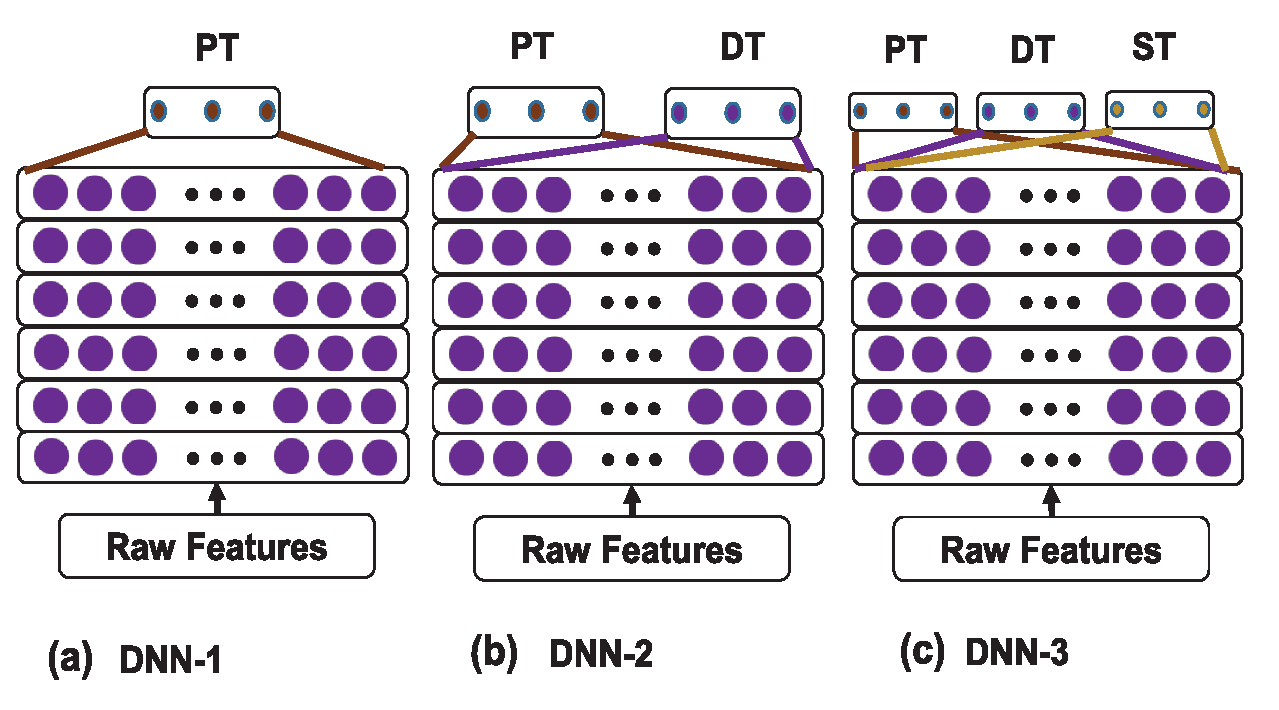
\includegraphics[width=\linewidth,height=5cm,keepaspectratio]{fig/DNN_multisoftmax.eps}
 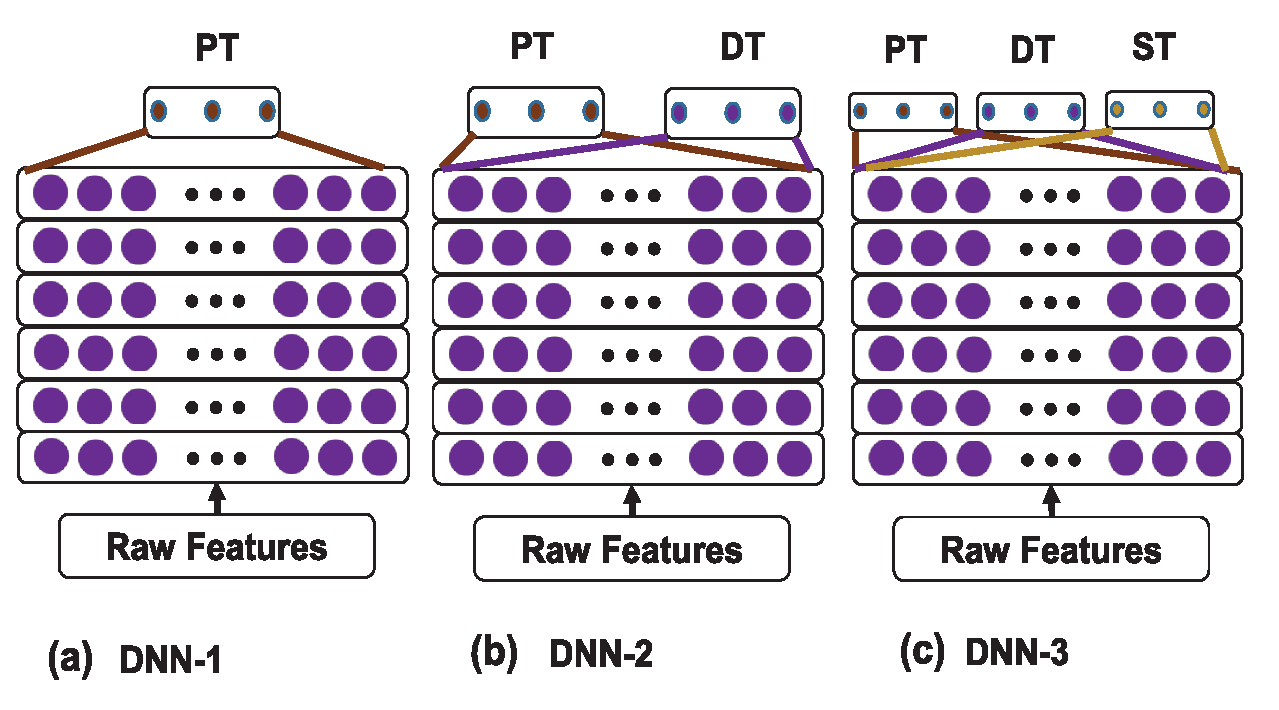
\includegraphics[width=\linewidth,height=5cm]{fig/DNN_multisoftmax.eps} 
 \myvspacefig
  \caption{DNN adaptation using probabilistic transcripts (PT).}
 \label{fig:DNN}
\end{figure}

\subsection{Probabilistic Error Rate}
\label{sec:Probabilistic Error Rate}
The aforementioned sections computed the phone error rates by measuring the edit distance between the 1-best path in the ASR decoding lattice and the reference DT. Hence, they may be considered as deterministic PERs. Our assumption was that there were no DTs in the target language in the training stage. Thus, it is fair to assume that there may not be DTs in the target language in the testing stage as well. An obvious question is how do we evaluate ASR systems for the target language in the absence of DTs? In the absence of DTs, we consider PTs to serve as a proxy for the reference ground truth labels. We denote the edit distance between the 1-best path in the ASR decoding lattice and the PTs as probabilistic phone error rate (PPER).
%We compute two different kinds of PPER - unweighted PPER (U-PPER) and weighted PPER (W-PPER). U-PPER is computed as follows. First, the PTs are pruned to retain the most reliable transcripts. Next, the probabilities on the arcs of the pruned PTs are stripped making the PT unweighted. Finally, the edit distance between the 1-best path in the ASR decoding lattice and the unweighted pruned PT is computed. For W-PPER, the only change is that the probabilities on the arcs of the pruned PTs are retained.
This is calculated as follows. First, the PTs are pruned to retain the most reliable transcripts. Next, the probabilities on the arcs of the pruned PTs are stripped making the PTs unweighted. Finally, the edit distance between the 1-best path in the ASR decoding lattice and the unweighted pruned PT is computed. The PPERs are reported in Table \ref{Tab:PPER}. Comparing the MAP-HMM and the MULTI systems, the absolute decrease in PPER in Table \ref{Tab:PPER} correlates well with the absolute decrease in PER in Table \ref{Tab:PER_PT} (refer to the second elements in parentheses under the column MAP-HMM). In addition, the PPER of DNN-2 also outperforms the MULTI system. (However, as opposed to the behavior in PER, the PPER of DNN-2 is higher than MAP-HMM.) Thus, PPERs allow us to correlate the improvements of the adapted systems over the unadapted ones; these improvements are verified to be accurate by PER computations in Table~\ref{Tab:PER_PT}.

%using PPER, we can correlate the improvements of the adapted system (MAP-HMM) over the unadapted ones (MULTI).

\begin{table}
\centering %\begin{center} does the same thing as \centering but inserts an extra line
\begin{tabular}{l|c c c}
   \hline
Lang  & \multicolumn{2}{c}{PPER (\%)} \\
          &  MULTI - MAP-HMM & MULTI - DNN-2  \\ \hline
swh      &  ??-??=?? & ?? - ?? = ??  \\
amh      & 64.46 - 57.16 = 7.3   & 64.46 - 59.80 = 4.67  \\ 
din     &64.09 - 58.59 = 5.5   &64.09 - 60.64 = 3.45 \\ \hline
\end{tabular}
\caption{Probabilistic Phone Error Rates} \label{Tab:PPER}
\vspace{-5mm}
\end{table}

\vspace{-3mm}
\section{Conclusions}
In this study, we presented a complete set of ASR training methods to train HMM and DNN systems using no deterministic but only probabilistic transcripts in Swahili, Amharic, and Dinka. We reported absolute phone error rate improvements of the PT adapted systems in the range 6.56\%-18.14\%. In addition, we found improvements in probabilistic error rates can correlate well with the improvements in deterministic phone rates. This is useful in the absence of deterministic transcripts in the test set.

% To start a new column (but not a new page) and help balance the last-page
% column length use \vfill\pagebreak.
% -------------------------------------------------------------------------
%\vfill
%\pagebreak

\clearpage
\newpage
\eightpt
\bibliographystyle{IEEEtran}
\bibliography{IEEEabrv,IEEEexample}

%  \begin{thebibliography}{9}
%    \bibitem[1]{Davis80-COP}
%      S.\ B.\ Davis and P.\ Mermelstein,
%      ``Comparison of parametric representation for monosyllabic word recognition in continuously spoken sentences,''
%      \textit{IEEE Transactions on Acoustics, Speech and Signal Processing}, vol.~28, no.~4, pp.~357--366, 1980.
%    \bibitem[2]{Rabiner89-ATO}
%      L.\ R.\ Rabiner,
%      ``A tutorial on hidden Markov models and selected applications in speech recognition,''
%      \textit{Proceedings of the IEEE}, vol.~77, no.~2, pp.~257-286, 1989.
%    \bibitem[3]{Hastie09-TEO}
%      T.\ Hastie, R.\ Tibshirani, and J.\ Friedman,
%      \textit{The Elements of Statistical Learning -- Data Mining, Inference, and Prediction}.
%      New York: Springer, 2009.
%    \bibitem[4]{YourName16-XXX}
%      F.\ Lastname1, F.\ Lastname2, and F.\ Lastname3,
%      ``Title of your INTERSPEECH 2016 publication,''
%      in \textit{Interspeech 2016 -- 16\textsuperscript{th} Annual Conference of the International Speech Communication Association, September 8–12, San Francisco, California, USA, Proceedings, Proceedings}, 2016, pp.~100--104.
%  \end{thebibliography}

\end{document}
